\newpage
\begin{multicols}{2}
\begin{wraptable}
\resizebox{5,5cm}{!}{

\begin{tabular}{|c| c| c| c| c|}
\hline
12 & 13 & 14 & 15 & 23 \\
\hline
24 & 25 & 34 & 35 & 45 \\
\hline
123 & 124 & 125 & 134 & 135 \\
\hline
145 & 234 & 235 & 245 & 345 \\
\hline
\end{tabular}
}

\quadТабл. 1

\end{wraptable}

\quad 

этому\\

$-\frac{1}{3}$ $\sum$ $M_{ijkl}$ + $\frac{2}{3}$ $M_{12345}$\leq0.

Теперь уже легко получить требуемый ответ. Из (7) следует, что\\

$\sum$$M_{ij}$ \geq 2\sum $M_{i}$ - 3M \geq

           \qquad    \qquad     \qquad           \geq 2 (5 \cdot \frac{1}{2}) - 3 = 2.\\

\noindent Но так как общее число «попарных пересечений заплат» $M_{ij}$ равно 10, то хоть одно из них не меньше чем   
$$2:10=\frac{1}{5},$$
что и требовалось доказать! 

Нетрудно видеть, что равенство здесь будет иметь место лишь тогда,
когда S = М, то есть когда кафтан весь покрыт заплатами, когда все
$M_{i}$ = 1/2, все M, одинаковы (и равны 1/5) и когда все $M_{ijkl}$ = 0. На рисунке 1 приведена схема покрытия кафтана заплатами, где прямоугольник М - это кафтан и цифры на отдельных квадратиках указывают, какими заплатами покрыты соответ-ствующие участки кафтана. Эта схема показывает, что 1/5 - точная оценка. То, что на ней заплаты состоят из отдельных кусков не должно вас кусков, не должно вас смущать - в задаче М185 важна только площадь заплаты, а не ее форма.
Теперь мы можем сформулировать общую задачу, частным случаем которой является задача М185:
\\
\\
\\
\textbf{Формулировка общей задачи;\\случай двух заплат}

\small
\textit{На кафтане М площади 1 имеется n заплат $M_{1}$, $M_{2}$, . . ., $M_{n}$, площадь каждой из которых не меньше известого нам числа $\alpha$; требуется оценить площадь наибольшего из пересечений $M_{ij}$ заплат}.\par
Другими словами, для каждой конфигурации из n заплат на кафтане мы находим м а к с и м а л ь н о е по площади пересечение $M_{ij}$, а потом отыскиваем м и н и м у м этого максимума $M_{ij}$ по всем возможным конфигурациям заплат *). Такого рода «минимаксные» (то есть связанные с нахождением минимума некоторых максимумов) задачи играют в современной математике очень большую роль.
\parИскомое число min max $M_{ij}$ зависит, разумеется, от заданного числа $\alpha$, то есть является функцией от $\alpha$; так как оно зависит также и от числа n заплат, то мы обозначим эту функцию через $f_n(\alpha)$ (где, очевидно, $0\leq$ \alpha $ \leq$ 1, а n $\geq$ 2). Решение задачи М185 сводится к доказательству равенства
$$f_5(\frac{1}{2}) = \frac{1}{5};$$
общая задача требует указать формулу, выражающую $f_n(\alpha)$ через $\alpha$ и n.

\small
Для того чтобы понять, какого ответа можно ожидать в этой общей задаче, мы начнем с (совсем простого!) случая n = 2. Итак, мы считаем, что на кафтане М площади 1 имеются д в е заплаты $M_{1}$ и $M_{2}$, площадь каждой из которых не меньше $\alpha$; нам надо указать наименьшую возможную площадь $f_2(\alpha)$ пересечения $M_{12}$ этих двух заплат.

Ясно, что если $\alpha$ ≤ 1/2, то заплаты, то наименьшая возможная площадь  $f_2(\alpha)$ пересечения
\rule[1mm]{60mm}{.1pt}\\
    \indent
    \small
    *) Мы предполагаем, что такой минимум существует, хотя это далеко не очевидно.\par
    \small





\end{multicols}

\begin{multicols}{2}
\newpage
  

\begin{wrapfigure}  
\centering
        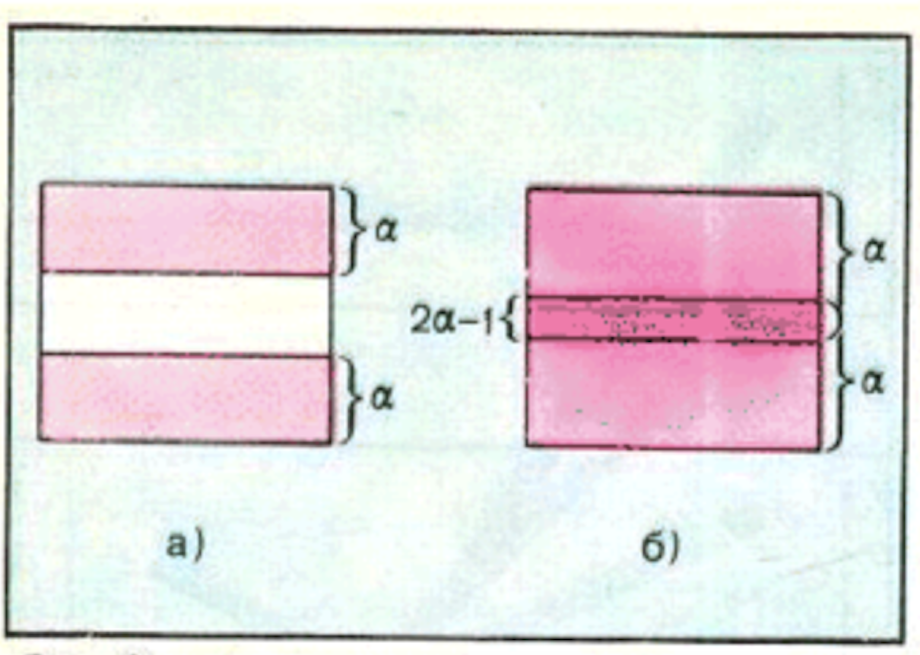
\includegraphics[width=.95\columnwidth]{latex.png}
\end{wrapfigure}

$M_{12}$, заплат равна 2$\alpha $ - 1 (рис. 2,б).
\\
\\Таким образом,   

\\и $M_{5}$, на кафтане М, про которые мы теперь будем считать, что\quad \qquad п л о щ а д ь\quad  к а ж д о й\quad  з а п л а т ы\quad  н е\quad м е н е е\quad $\alpha$. Наша задача состоит в том, чтобы определить функцию $f_5(\alpha)$.

Прежде всего ясно, что $f_5(\alpha)$. ≥  0 - график функции у = $f_5(\alpha)$.
лежит не ниже оси у = 0. (рис. 5)
Для того чтобы наш график совпал с осью, то есть чтобы было возможно обращение всех $M_{ij}$ в 0, очевидно, необходимо (и достаточно), чтобы общая площадь всех заплат (по условию задачи не меньшая 5$\alpha$ не превосходила площади 1 кафтана:

\end{multicols}

